This chapter is dedicated to providing the theoretical foundations behind our benchmark. We discuss here the main problems that underlie our work; in particular, we introduce the idea of security protocol, along with our notation for expressing message exchanges in Section~\ref{sec:securityprotocols}. In Section~\ref{sec:formalverification}, we discuss the problem of formal verification, highlighting the main techniques developed for it and how this task has been tackled in the field of computer-aided cryptography.


\section{Security Protocols}
\label{sec:securityprotocols}

In this section we provide an introduction to security protocols: in Section~\ref{sec:historyofcommunication} we present a brief overview of the history of cryptographic schemes, from their ancient origins up to today's standards. In Section~\ref{sec:dolevyao} we introduce Dolev Yao's model, which is the foundational framework used in formal methods research for verifying the properties of such protocols.

\subsection{Brief History of Communication Protocols}
\label{sec:historyofcommunication}

Cryptographic protocols feature a long and rich history, dating back to ancient civilizations, where basic forms of encryption were used to secure strategic communications. Although the quick development and adoption of cryptographic protocols as we intend them today began only during the mid-20th century after the advent of electronic systems, mathematicians have been engineering encryption schemes (mostly for war-related reasons) since the Roman Empire.

The earliest known cryptographic technique, the \textit{Caesar Cipher}, was used by Julius Caesar to protect his military communications. This simple substitution cipher involved shifting each letter of the plaintext by a fixed number of places down the alphabet and, even if it was easy to break, it laid the groundwork for the development of more sophisticated methods of securing information during the following centuries.

The \textit{Enigma machine}, used by the Germans during World War II to prevent eavesdropping on military communications, represents another significant milestone in the history of cryptography. The machine-implemented a polyalphabetic substitution cipher, which guaranteed substantial security for its time. The breakage of its encryption scheme by Alan Turing and his team at Bletchley Park deeply influenced the rest of the war and laid the foundation of computational cryptography.

We can locate the birth of modern cryptographic protocols in the 1970s, corresponding with the invention of \textit{public-key cryptography} by Whitfield Diffie and Martin Hellman~\cite{newdirections}. Their paper introduced the concept of asymmetric encryption, where two separate keys (one public and one private) can used for encryption and decryption. In the eighties cryptographic protocols expanded beyond simple encryption schemes to include more complex systems for securing communications. \textit{Merkle's puzzles}~\cite{merklepuzzle}, the \textit{Diffie-Hellman exchange} (explained in the same article where they introduced asymmetric encryption) and the \textit{Needham-Schroeder protocol}~\cite{needhamschroeder} are some of the most famous exchanges developed in those years to address the critical issue of key distribution across insecure channels. Correcting the flaws of these protocols laid the groundwork for the development of even more advanced cryptographic schemes, such as the \textit{Kerberos authentication system}~\cite{kerberos} and the \textit{Transport Layer Security protocol}~\cite{tls} (TLS), which are widely used today to provide trustworthy distributed authentication mechanisms and secure web traffic.

A \textit{cryptographic protocol} consists of a distributed algorithm, generally expressed as a sequence of computational steps, that two or more parties execute to achieve a specific security goal, such as confidentiality, integrity, authentication, or non-repudiation. Protocol steps may involve the use of cryptographic primitives, such as symmetric encryption algorithms or digital signatures, to enforce security and avoid tampering from a malicious party. In particular, when we specify a cryptographic protocol, we generally have to declare:
\begin{itemize}
    \item \textbf{Participants}. The entities involved in the communication.
    \item \textbf{Messages}. The content exchanged between participants.
    \item \textbf{Assumptions}. The initial conditions or trust relationships assumed to hold, such as the secure generation of keys, the reliability of cryptographic primitives and the initial knowledge of the participants.
    \item \textbf{Security Properties}. The properties the protocol tries to guarantee, such as secrecy of the messages, integrity of the communication, and verification of the identities of the participants.
\end{itemize}

Security protocols are validated based on their ability to resist to various types of attacks, which can range from passive eavesdropping to active manipulation or impersonation by malicious entities. It is no surprise that attack techniques have evolved over the years to keep up with an increase in protocol complexity. Initially, malicious parties mainly focused on breaking cryptographic primitives, such as ciphers and hash functions, through brute force and mathematical analysis. As these primitives became more secure, attackers shifted their focus to exploiting weaknesses in the logic of the protocols themselves, searching for effective attack vectors agnostic to the implementations of the cryptographic operations.

One of the earliest examples of an attack on a protocol's logic is the \textit{man-in-the-middle attack} (MitM) on the Diffie-Hellman key exchange, where an adversary intercepts and alters the messages between two parties, allowing him to secretly establish a shared key with both participants and freely access the following communication. The pair of protocols introduced by Needham and Schroeder in 1978~\cite{needhamschroeder} is another famous example of a logical flaw that was discovered years after its introduction. In the paper, the authors present two variants of the same cryptographic protocol, one based upon symmetric encryption, and the other one based on public-key cryptography, designed to exchange keys between two parties securely. Three years later, the symmetric key variant was found to be vulnerable to replay attacks, and quickly fixed with the introduction of timestamps under the name of \textit{Denning and Sacco protocol}~\cite{denningsacco}. Interestingly enough, the other variant featured a similar flaw that was not discovered until 14 years later, leading to a plethora of unsafe implementations worldwide. After the necessary modifications, it is now known as the \textit{Needham-Schroeder-Lowe protocol}.

The discovery of flaws in cryptographic protocols can have severe consequences: if exploited, these vulnerabilities can lead to unauthorized access to sensitive information, impersonation of users, or the ability to manipulate data undetected. For example, a compromise of the SSL/TLS protocol through attacks like BEAST~\cite{beast} or POODLE~\cite{poodle} would allow attackers to decrypt confidential communications, potentially leading to the exposure of passwords, financial information, or private messages. As a consequence, it is crucial to carefully validate protocols before deploying them into production. In Section~\ref{sec:formalverificationcrypto} we investigate this matter further, explaining the computational issues behind verifying the absence of attacks in new protocols.

\subsection{Dolev Yao's Model}
\label{sec:dolevyao}

The Dolev Yao model, introduced by Danny Dolev and Andrew Yao in 1983~\cite{dolevyao}, is a symbolic framework used to analyze the security of cryptographic protocols. It represents one of the foundational models in the field of defensive cybersecurity, as it provides a set of reasonable assumptions to formally verify the absence of attacks in protocols. The main feature of this model consists of the abstraction of cryptographic operations into symbolic terms, allowing computer scientists to carefully inspect the protocol logic through algebraic methods, ignoring the intricacies of the actual implementations.

In the paper, we can identify 4 main assumptions, that represent the core of this framework's symbolic nature. Unfortunately, the original work was intended only to investigate asymmetric-encryption cryptosystems, and thus is not directly applicable to protocols that feature different primitives, such as Exclusive-OR, digital signatures or Diffie-Hellmann exponentiation. As a consequence, we now present the original assumptions, along with some reasonable extensions (often already implicitly used in the current literature) that allow us to analyze a broader class of protocols.

\paragraph{\textbf{Perfect Cryptography Assumption}.} The original model assumes one-way functions to be unbreakable, private keys to be secret and public keys to be known and usable to everybody, but never tampered with. In practice, this entails that an attacker cannot decrypt an encrypted message without the proper key. We generalize this idea by postulating that cryptographic operations work according to strict semantics expressed by a predetermined set of symbolic identities (the reader can consult Section~\ref{sec:formalizingmessages} for further reference). An attacker can not invalidate this hypothesis under any circumstance and thus is not able to exploit design or implementation flaws in the primitives themselves. Furthermore, we lift the requirement of public keys to be necessarily known to everyone, as we might want to analyze, for example, protocols for certificate authorities or public directories.

\paragraph{\textbf{Local Encryption}.} Dolev Yao's model assumes the various participants to be capable of locally executing encryption and decryption algorithms, without relying on external parties for cryptography operations. We relax this assumption by including all primitives involved in a protocol. Furthermore, we assume all cryptographic primitives to be deterministic, excluding probabilistic schemes. This facilitates the formal verification of the protocols, as the behavior of each operation is predictable and consistent.

\paragraph{\textbf{Closed World Assumption}.} The original model operates under the closed-world assumption, where all possible protocol actions and message formats are predefined. This implies that the adversary cannot introduce new, unforeseen message formats or operations into the protocol, as they would get detected by the honest participants. In practice, this implies that the various parties perform all checks made possible by their knowledge to verify the authenticity of the messages they receive from the network. The protocol’s security is therefore analyzed within the constraints of the defined message space, simplifying the reasoning process.

\paragraph{\textbf{Ubiquitous Adversarial Model}.} The Dolev Yao model assumes a ubiquitous adversary with complete control over the communication medium. In particular, the adversary can intercept, modify, inject, or block any message sent between the protocol participants: in other words, "the attacker carries the message". This adversarial model allows researchers to ensure that the protocol remains secure even under the most adverse conditions by assuming the worst-case scenario during protocol verification.

\vspace{10pt}

When working under Dolev Yao's assumptions, protocols are often specified in \textit{Alice and Bob} (AnB) notation. It features a simple and intuitive syntax, that abstracts protocols to sequences of algebraic messages exchanged between parties. An example of the Needham Schroeder protocol expressed in this notation is provided in Figure~\ref{fig:needhamschroedersimplified}.

\begin{figure}[htbp]
    \centering
    \begin{align*}
        A \to S &: \langle A, B, N_A \rangle\\
        S \to A &: \texttt{senc}(\langle N_A, K_{AB}, B, \texttt{senc}(\langle K_{AB}, A \rangle, K_{BS}) \rangle, K_{AS})\\
        A \to B &: \texttt{senc}(\langle K_{AB}, A \rangle, K_{BS})\\
        B \to A &: \texttt{senc}(N_B, K_{AB})\\
        A \to B &: \texttt{senc}(N_B - 1, K_{AB})
    \end{align*}
    \caption{The Needham Schroeder Symmetric Key Protocol, expressed in Alice and Bob notation. Note that, although this syntax is very straightforward and intuitive, when reading this example we must make a series of deliberate assumptions about the initial knowledge of the parties. For example, we have to take for granted that $A$ and $B$ both know the shared key $K_{AB}$, which is reasonable in this scenario, however it is not always the case.}
    \label{fig:needhamschroedersimplified}
\end{figure}

Unfortunately, as pointed out in 2006 by Caleiro et al.~\cite{anbsemantics}, in its simplest form AnB is an inherently ambiguous language, which is not always suitable for formal verification. As a consequence, even if most of the examples in this thesis are expressed like in Figure~\ref{fig:needhamschroedersimplified} for succinctness, in our benchmark we adopt an extension of AnB that requires explicit function, knowledge and fresh messages declarations. The grammar that generates this language, along with an example protocol, is provided in Figure~\ref{fig:anbgrammarexample}.

\begin{figure}[htbp]
    \centering
    \begin{minipage}{0.8\textwidth}{\small
        \centering
        \begin{align*}
            \text{Protocol} &::= \texttt{Protocol : } \textit{Identifier} \ \text{Declarations}? \text{ Knowledge}? \text{ Actions Goals}?\\
            \text{Declarations} &::= \texttt{Declarations : } ((\texttt{public} \ | \ \texttt{private}) \ \textit{Identifier}/\textit{Number};)^{*}\\
            \text{Knowledge} &::= \texttt{Knowledge : } (\text{Agent} : (\text{Msg}(,\text{Msg})^{*}) ;)^{*}\\
            \text{Actions} &::= \texttt{Actions : } ([\textit{Identifier}] \ \text{Agent} \to \text{Agent} \ \texttt{(}\text{Msg}(,\text{Msg})^{*}\texttt{)}? : \text{Msg};)^{+}\\
            \text{Agent} &::= \textit{Identifier}
        \end{align*}}
        \subcaption{Context-free grammar in Extended Backus-Naur form~\cite{ebnf} for the extended AnB. Note that the terminal leaves are italicized, whereas strings are written in monospaced font. All the other terms are production symbols. The grammar for the encrypted messages and goals is not defined here since it depends on the primitives involved in the protocol and its security properties.}
        \label{fig:anbgrammar}
    \end{minipage}
    \hfill
    \begin{minipage}{0.8\textwidth}{\small
        \begin{align*}
            &\texttt{Protocol : } \text{Needham Schroeder Symmetric Key Protocol}\\
            &\texttt{Declarations : }\\
            &\ \ \ \ \texttt{public senc}/2;\\
            &\texttt{Knowledge : }\\
            &\ \ \ \ A : K_{AS};\\
            &\ \ \ \ B : K_{BS};\\
            &\texttt{Actions : }\\
            &\ \ \ \ [ns1] \ A \to S \ (N_A) : \langle A, B, N_A \rangle\\
            &\ \ \ \ [ns2] \ S \to A \ (K_{AB}) : \texttt{senc}(\langle N_A, K_{AB}, B, \texttt{senc}(\langle K_{AB}, A \rangle, K_{BS}) \rangle, K_{AS})\\
            &\ \ \ \ [ns3] \ A \to B \ : \texttt{senc}(\langle K_{AB}, A \rangle, K_{BS})\\
            &\ \ \ \ [ns4] \ B \to A \ (N_B) : \texttt{senc}(N_B, K_{AB})\\
            &\ \ \ \ [ns5] \ A \to B \ :\texttt{senc}(N_B - 1, K_{AB})
        \end{align*}}
        \subcaption{The Needham Schroeder Symmetric Key Protocol, in extended AnB notation. Note that each freshly generated term is declared in parentheses before its sending.}
        \label{fig:needhamschoredercomplicated}
    \end{minipage}
    \caption{The extended AnB notation. In Figure~\ref{fig:anbgrammar} we propose a partial description of the grammar that defines the language, while in Figure~\ref{fig:needhamschoredercomplicated} we show how the example of the Needham Schroeder protocol becomes less ambiguous in this notation.}
    \label{fig:anbgrammarexample}
\end{figure}

The same set of assumptions that determines the strength of the Dolev Yao model is also its main source of weakness. Abstracting cryptographic operations to symbolic terms allows the application of algebraic methods for verification, but, on the other hand, ignores all the potential flaws that may arise from incorrect implementation. Consequently, many protocols that rely on complex custom primitives (such as Zero-Knowledge proofs) are generally analyzed more naturally in another threat model, the \textit{computational model}. Since this thesis aims to investigate the possibility of AI-based verification software to validate large-scale protocols, where logical flaws may be harder to identify, Dolev Yao's model is the better choice.

\clearpage

\section{Formal Verification}
\label{sec:formalverification}
Verification is a critical area in computer science focused on ensuring that systems behave according to their specified requirements. As software and hardware systems become increasingly complex and integral to critical scenarios, such as in aerospace, medical devices, and cryptographic protocols, the need for guaranteed reliability has never been more essential. There are four classes of methods that are implemented for verification in Computer Science: \textit{simulation}, \textit{testing}, \textit{deductive verification} and \textit{model checking}.

Simulation and testing both consist of ensuring that a system behaves according to its specifications for a comprehensive set of scenarios. The main difference between the two methods lies in the fact that, while simulation is performed on an abstraction of the system, testing is carried out directly on the product. These approaches provide empirical evidence that a system is ready for deployment and is generally easy to implement, although they do not guarantee that a product will never deviate from the specification.

In the past, there have been several occasions where critical systems faced unexpected, catastrophic failures due to improbable circumstances not anticipated during testing/simulation. Some examples are the floating-point division bug found in Intel Pentium processors, which caused an estimated loss of \$475 million to the company~\cite{pentiumbug}, or the crash of the Ariane 5 rocket in 1996~\cite{ariane5}. When dealing with critical systems, it is thus important to apply other kinds of techniques to avoid such accidents by ensuring that certain harmful behaviours never occur.

The latter two approaches in our list are considered methods of \textit{formal verification} and aim at proving that a system will follow its specification under all circumstances. Deductive verification techniques employ axioms and proof rules to guarantee that certain properties are satisfied during all possible executions of a system. This approach allows reasoning on infinite-state systems but can be automated only to a limited extent. On the other hand, model checking performs an exhaustive exploration of the state space of a system, automatically verifying that a specification is never contradicted. Both of these approaches produce interpretable counterexamples when the verification procedure terminates unsuccessfully, providing valuable information for fixing a system under development.

In the following sections, we discuss the main formal verification approaches, beginning with an exploration of model checking, followed by an examination of deductive reasoning techniques. After providing a more precise introduction to the main techniques, we investigate the application of formal verification in the domain of cryptographic protocols, where proof of correctness is crucial for safe deployment.

\subsection{Model Checking}

Model checking is a formal verification technique designed to exhaustively explore the state spaces of complex computational systems to ensure that they satisfy a given set of input properties~\cite{stateexplosion}. This approach was initially developed in 1982 by Clarke and Emerson~\cite{modelchecking} as a technique to mechanize the synthesis of finite-state systems, such as concurrent programs running in a shared-memory environment and distributed algorithms. In particular, the primary motivation behind model checking is to provide a rigorous and automated approach for detecting errors in complex and critical systems before they are deployed, thereby improving their reliability and safety. 

At its core, model checking involves three key components: an abstract representation of the system, a property to verify, and a verification algorithm. Formally, the problem can be defined as follows: given an abstract model $M$ and a specification $\phi$ expressed in a formal logic, the goal is to determine whether the model satisfies the specification, denoted as $M \models \phi$. The outcome of the verification procedure is either a confirmation that the system will never deviate from its specification or a valid execution trace that satisfies $\neg \phi$.

The model $M$ is often represented as a labelled transition system, or a Kripke structure $M = (S, S_0, R, L)$, where
\begin{itemize}
    \item $S$ is a finite set of states.
    \item $S_0 \subseteq S$ is a set of initial states.
    \item $R \subseteq S \times S$ is a transition relation, defining all possible evolutions of the state.
    \item $L: S \rightarrow 2^{AP}$ is a labeling function that assigns to each state a set of atomic propositions from a set $AP$, that is true in that state.
\end{itemize}
The \textit{model} is an abstract representation of the system under verification, capturing the possible states the system can be in and the transitions between those states. The accuracy and completeness of the model are crucial, as any omission or incorrect detail can lead to invalid verification results. The \textit{state space} is the collection of all possible states that a system can assume during its execution, along with the transitions between these states. In model checking, the state space is typically finite, though it can be very large, as it grows exponentially concerning the number of variables used in the system. This problem is known as \textit{state explosion}~\cite{stateexplosion}. The \textit{transition relation} defines how the system evolves from one state to another. This relation is a critical part of the model, as it encodes the causal dependencies between states. In complex models, transitions may be labelled with actions or conditions that must be met for the transition to occur (analogously to the symbols on the edges of finite automata). The \textit{labelling function} assigns a set of atomic propositions to each state in the model. These propositions encode basic facts about the system that are true in that state. For example, a proposition might indicate whether a particular variable has a specific value or whether a process is in a particular mode. The labelling function is required to interpret the states of the model in terms of the properties to verify.

The language to express $\phi$ may vary based on the nature of the model, but it often consists of some fragment of temporal logic, such as Linear Temporal Logic (LTL) or Computation Tree Logic (CTL). These logics can naturally describe temporal properties that the system must satisfy during its evolution~\cite{temporallogics}. For example, an LTL formula for a distributed system might specify that "every request will eventually be followed by a grant", ensuring deadlock prevention.

The model-checking algorithm explores the state space of the model $M$ to verify whether the specification $\phi$ holds for all possible execution paths. This generally involves an exhaustive exploration, where the algorithm systematically traverses states and transitions in the model according to $R$. As we explained before, the state space of a model may suffer from state explosion, leading to computationally intensive verification procedures in the case of naive algorithms. However, researchers have observed that multiple symmetries in a model can be exploited to speed up the verification procedure. In parallel, another technique has been developed to handle huge state spaces through symbolic manipulation: the idea of \textit{symbolic model checking} was introduced in 1992 by McMillan et al.~\cite{symbolicmc}. Instead of explicitly enumerating all possible states and transitions in a system, symbolic model checking represents the state space using mathematical structures like Binary Decision Diagrams (BDDs) or, more generally, symbolic expressions over boolean variables. For example, rather than listing all possible values of a counter in a system, symbolic model checking can use a formula to represent the entire range of possible values. Such a representation allows the model checker to manipulate sets of states and transitions compactly, often resulting in significant reductions in memory usage and computational effort. This approach not only allows for the verification of huge models but is also able to handle systems with infinite state spaces, as logical formulas can represent infinite sets of states.

This approach is particularly useful for verifying properties of applications that operate over potentially infinite domains, such as cryptographic protocols with unbounded message sizes or counters. By leveraging symbolic representations, it is possible to reason about all possible behaviours of the protocol without having to explicitly construct and traverse an infinite state space.

\subsection{Deductive Reasoning}

Deductive reasoning plays a central role in formal verification, offering a rigorous approach to proving that systems adhere to their specified properties. In particular, deductive reasoning aims to verify correctness through logical inference, ensuring that a system behaves as intended in all possible scenarios. Deductive reasoning tools provide the frameworks necessary to conduct these rigorous analyses, enabling the formalization and verification of complex systems with potentially infinite state space.

In the field of computer science, the problem of deductive reasoning can be formally stated as follows: given a system $S$ described by a set of logical formulas $\Phi$, and a property $P$ that the system is expected to satisfy, the objective is to prove that $\Phi \vdash P$, where $\vdash$ denotes logical entailment. In other words, the goal is to show that the property $P$ is a logical consequence of the system's specification $\Phi$. The challenge of deductive reasoning lies in constructing a proof that $P$ holds for all possible executions or configurations of the system. Since proofs are often hard to derive, researchers have tried to develop automatic techniques to handle this problem, but, unfortunately, deductive reasoning generally is used to tackle inherently undecidable problems. As a consequence, there can not be any general procedure to always determine whether a statement derives from a set of axioms. As of today, two main categories of tools can be identified: \textit{proof assistants} and \textit{theorem provers}.

\paragraph{\textbf{Proof Assistants}.}
Proof assistants are tools designed to assist users in constructing formal proofs by providing a framework for defining logical theories, stating theorems, and incrementally building proofs. These tools combine automation with user interaction, allowing users to apply logical tactics and strategies to guide the proof process. They generally feature a particular component, called the \textit{kernel}, which checks the validity of each step of the proofs.  A proof-deriving program can be at most trustworthy as its kernel. Since correctness (and trust) within this field is critical, many proof assistants feature simple and well-specified kernels, developed and distributed independently of the overall architecture. This choice follows \textit{de Bruijn criterion} for deductive reasoning: in the words of Barendregt and Wiedijk~\cite{challengeofmaths},

\begin{displayquote}
Indeed a verifying program only needs to see whether in the computative proof, the small number of logical rules are always observed. Although the proof may have the size of several Megabytes, the verifying program can be small. This program then can be inspected in the usual way by a mathematician or logician. If someone does not believe the statement that a proof has been verified, one can do independent checking by a trusted proof-checking program. [...] A Mathematical Assistant satisfying the possibility of independent checking by a small program is said to satisfy the de Bruijn criterion.
\end{displayquote}

Proof assistants are highly expressive, and support complex reasoning and higher-order logic, which makes them suitable for verifying intricate systems that require detailed, step-by-step proof construction. In particular, such tools work by allowing users to define mathematical structures, specify the properties of these structures, and interactively develop proofs. The user guides the proof process by applying logical inference rules, while the proof assistant handles routine steps and checks the validity of each deduction. This is especially helpful when writing logical proof that requires considering many edge cases. The writer of the proof can feel assured by the tool not to have forgotten any hidden detail, while the reader can avoid checking the whole proof by only reading the initial statement and trusting the kernel.

Proof assistants are used because they offer a high degree of flexibility and control over the proof process, allowing users to tackle complex verification tasks. Two famous long-standing problems that were eventually solved with the help of proof assistants were the four-colour theorem (every planar graph allows a proper vertex colouring with four colours)~\cite{fourcolor} and Kepler's conjecture (no arrangement of equally sized spheres filling space has a greater average density than that of the cubic close packing and hexagonal close packing arrangements)~\cite{keplerconjecture}. More generally, proof assistants can be particularly valuable in fields such as mathematics, software correctness, and hardware verification, where the correctness of a system depends on intricate logical relationships. By enabling users to construct detailed and rigorous proofs, proof assistants provide a powerful tool for ensuring the reliability of critical systems.

Some examples of domain-agnostic proof assistants are \textit{Coq}~\cite{coq}, which is widely used for formalizing mathematical theories and verifying software, \textit{Isabelle/HOL}~\cite{isabelle}, used extensively in software and hardware verification, such as for the validation of the seL4 microkernel~\cite{seL4proof}, and \textit{Lean}~\cite{lean}, which is gaining popularity in both academic and industrial scenarios for its combination of powerful automation and user-friendly interface.

\paragraph{\textbf{Theorem Provers}.} Theorem provers are automated tools that focus on proving or disproving logical formulas with minimal user interaction. These tools attempt to derive proofs based on a set of axioms and inference rules, often using decision procedures, heuristics, and symbolic reasoning to explore the space of possible proofs. Theorem provers are designed to handle a wide range of verification tasks, from checking the validity of logical assertions to verifying properties of complex systems, including those with infinite state spaces. Early automated deduction systems were developed upon Herbrandt's Fundamental Theorem~\cite{herbrandtheorem}, which suggested how a sound and complete automatic deduction procedure could be built. Later on, also different approaches were explored for automatic reasoning tools, such as resolution refinement techniques~\cite{lovelandautomatic}, term rewriting algorithms~\cite{equationsandrr} and the inclusion of induction in theorem proving~\cite{combininginduction}. The reader may consult~\cite{surveyautomated} for a more comprehensive literature review regarding the history and evolution of these tools.

Theorem provers work by taking a formal specification of a system, along with a set of desired properties, and automatically exploring the logical consequences of these inputs. They use various strategies to search for proofs, including backtracking, resolution, and constraint solving. In particular, given the formula $\phi$, theorem provers often try to find a case that leads to $\neg \phi$, effectively checking for satisfiability instead of validity. If such a case is found, 
the theorem prover generally provides the counterexample that demonstrates the failure, analogously to model checkers. On the other hand, if a proof for $\phi$ is found, the tool can either return it or confirm that the property holds.

Theorem provers are used because they provide a high degree of automation, making them suitable for large-scale verification tasks where manual proof construction would be impractical, such as in software verification, automated reasoning, and symbolic computation. Some open problems that have been solved in the past with the assistance of automated deduction techniques are the \textit{Robbins Problem}~\cite{robbinsproblem}, along with a series of results in the field of equational logic (the reader can refer to Chapters 3 and 4 of~\cite{adequationallogic} for more information about said theorems). By automating the proof search process, theorem provers can (sometimes) handle complex verification tasks more efficiently than manual methods, making them an essential tool in formal verification.

Some examples of modern theorem provers are \textit{Z3}~\cite{z3}, a \textit{satisfiability modulo theories} prover developed by Microsoft Research used for software verification, computational biology, constraint solving and geometrical analysis, \textit{E Prover}~\cite{eprover}, created at TUM at the end of the 90s to provide a very efficient and effective higher order logic prover, and \textit{Vampire}~\cite{vampire}, which has been successfully applied to software verification and formal methods research.

While both proof assistants and theorem provers are essential tools in formal verification, they serve different purposes and operate in distinct ways. Proof assistants require significant user interaction, allowing for greater flexibility and control over the proof process. This makes them ideal for verifying complex systems where intricate logical reasoning and human insight are necessary. Theorem provers, on the other hand, are more automated and are designed to handle large-scale verification tasks with minimal user intervention. They are often successfully applied to restricted domains where the state space is vast, or the verification task lends itself to be automated using decision procedures and heuristics. However, the inherent complexity of the deductive problem in its broadest setting implies that such tools can only rarely obtain non-trivial results in more general scenarios.

\subsection{Formal Verification of Cryptographic Protocols}
\label{sec:formalverificationcrypto}

The increasing complexity of cryptographic protocols and the critical importance of their security have driven the development of computer-aided cryptography (CAC). This field leverages automated tools and formal methods to design, analyze, and verify cryptographic systems, ensuring their robustness against potential attacks. In particular, according to the 2019 survey on CAC published by Barbosa et al.~\cite{sok}, formal verification techniques can be helpful during all phases of deployment for new cryptosystems:

At the design level, tools can help manage the complexity of security proofs, even revealing subtle flaws or as-yet-unknown attacks in the process. At the implementation level, tools can guarantee that highly optimized implementations behave according to their design specifications on all possible inputs. At the deployment level, tools can check that implementations correctly protect against classes of side-channel attacks. Although individual tools may only address part of the problem, when combined, they can provide a high degree of assurance.

Researchers have developed various tools to assist with a wide set of problems belonging to the cryptography field. Applications range from verifying protocol drafts in the computational model, to validating new cryptographic primitives, to synthesizing provably correct implementations of cryptosystems from abstract specifications. However, in the remaining part of this section we restrict our scope to the verification of the security properties of cryptographic protocols in the symbolic model, as it represents the main objective of this thesis.

Verifying protocols according to Dolev Yao's assumptions is an infinite state space problem, as it features two sources of infinity: the number of executions of the protocol and the size of the messages considered. If we bound both, we restrict the problem to a finite-space problem, and thus we can apply standard model checking techniques. This approach has been implemented for the verifiers FDR~\cite{fdr} and SATMC~\cite{satmc}. Under reasonable assumptions, it can be shown that protocol insecurity is NP-complete even if we bound only the number of executions~\cite{boundedsessionsnp}: in practice, the verifier non-deterministically guesses a specific protocol execution, and then checks if it is a valid attack in polynomial time. Examples of verifiers that implement this technique are Cl-AtSe~\cite{clatse} and OFMC~\cite{ofmc}. Finally, if we avoid restricting the number of executions of the protocol, the problem becomes undecidable~\cite{complexitybounded}. Researchers have implemented different techniques to handle this issue within deductive reasoning tools: requiring user input (as in the case of Tamarin~\cite{TamarinFoundations} and Cryptyc~\cite{cryptyc}), producing inconclusive results (like in ProVerif~\cite{proverif} and the technique based on tree automata developed by Monniaux~\cite{monniaux}) or allowing non-termination (as in MAUDE-NPA~\cite{nrl, maude}).

The choice of verifier to use is generally mostly determined by the set of assumptions we are willing to work under. In some cases, we may decide that validating a protocol for a limited number of sessions is reasonable, while other times we might need to have better security guarantees (as in the case of widespread and/or critical protocols). However, we typically also want to take into consideration other features and limitations of the available tools when deciding. In particular, we might have to model a custom cryptographic primitive that features associativity or commutativity (AC). Or we might want to check equivalence properties to verify privacy statements, which are not supported by all tools within this field. Or we might want to verify a protocol with a global mutable state (as in the case of protocols that involve shared databases). Choosing the right verifier is not a trivial task and often requires some form of compromise. 
% \begin{figure}

%     \begin{minipage}{\textwidth}
%         \begin{adjustwidth}{-1in}{-1in}  
%         \centering
%         \rowcolors{3}{tableShade}{white}
%         \begin{tabular}{lcccccccccc}
%         \toprule
%         \textbf{Tool} & \textbf{Lang} & \textbf{Unbound} & \textbf{Trace} & \textbf{Equiv} & \textbf{Eq-thy} & \textbf{State} & \textbf{Inter} & \textbf{Verif} & \textbf{Abs}\\
%         \midrule
%         CPSA~\cite{cpsa} & $\CIRCLE$ & $\CIRCLE$ & $\CIRCLE$ & $\Circle$ & $\Circle$ & $\CIRCLE$ &  $\Circle$ & $\Circle$ & $\Circle$ \\
%         F7~\cite{f7} & $\Circle$ & $\CIRCLE$ & $\CIRCLE$ & $\Circle$ & $\LEFTcircle$ & $\CIRCLE$ &  $\Circle$ & $\Circle$ & $\Circle$ \\
%         $\expansion$F5~\cite{f5} & $\Circle$ & $\CIRCLE$ & $\CIRCLE$ & $\Circle$ & $\LEFTcircle$ & $\CIRCLE$  & $\Circle$ & $\Circle$ & $\Circle$ \\
%         Maude-NPA~\cite{maude} & $\CIRCLE$ & $\CIRCLE$ & $\CIRCLE$ & $\RIGHTcircle$ & $\CIRCLE$ & $\Circle$  & $\Circle$ & $\Circle$ & $\Circle$ \\
%         ProVerif~\cite{proverif} & $\LEFTcircle$ & $\CIRCLE$ & $\CIRCLE$ & $\RIGHTcircle$ & $\LEFTcircle$ & $\Circle$  & $\Circle$ & $\Circle$ & $\CIRCLE$ \\
%         $\expansion$fs2pv~\cite{fs2pv} & $\Circle$ & $\CIRCLE$ & $\CIRCLE$ & $\Circle$ & $\LEFTcircle$ & $\Circle$ & $\Circle$ & $\Circle$ & $\CIRCLE$ \\
%         $\expansion$GSVerif~\cite{gsverif} & $\LEFTcircle$ & $\CIRCLE$ & $\CIRCLE$ & $\Circle$ & $\LEFTcircle$ & $\CIRCLE$ & $\Circle$ & $\Circle$ & $\CIRCLE$ \\
%         $\expansion$ProVerif-ATP~\cite{proverifapt} & $\LEFTcircle$ & $\CIRCLE$ & $\CIRCLE$ & $\Circle$ & $\CIRCLE$  & $\Circle$ & $\Circle$ & $\Circle$ & $\CIRCLE$ \\
%         $\expansion$StatVerif~\cite{statverif} & $\LEFTcircle$ & $\CIRCLE$ & $\CIRCLE$ & $\RIGHTcircle$ & $\LEFTcircle$  & $\Circle$ & $\Circle$ & $\Circle$ & $\CIRCLE$ \\
%         Scyther~\cite{scyther} & $\CIRCLE$ & $\CIRCLE$ & $\CIRCLE$ & $\Circle$ & $\Circle$ & $\Circle$  & $\Circle$ & $\Circle$ & $\Circle$ \\
%         scyther-proof~\cite{scytherproof} & $\CIRCLE$ & $\CIRCLE$ & $\CIRCLE$ & $\Circle$ & $\Circle$ & $\Circle$  & $\CIRCLE$ & $\CIRCLE$ & $\Circle$ \\
%         Tamarin~\cite{TamarinFoundations} & $\RIGHTcircle$ & $\CIRCLE$ & $\CIRCLE$ & $\RIGHTcircle$ & $\CIRCLE$ & $\CIRCLE$  & $\CIRCLE$ & $\Circle$ & $\Circle$ \\
%         $\expansion$SAPIC~\cite{sapic} & $\LEFTcircle$ & $\CIRCLE$ & $\CIRCLE$ & $\Circle$ & $\CIRCLE$ & $\CIRCLE$ & $\Circle$ & $\Circle$ & $\Circle$ \\
    
%         \hdashline
    
%         Cl-AtSe~\cite{clatse} & $\CIRCLE$ & $\Circle$ & $\CIRCLE$ & $\Circle$ & $\CIRCLE$ & $\CIRCLE$ & $\Circle$ & $\Circle$ & $\Circle$ \\
%         OFMC~\cite{ofmc} & $\CIRCLE$ & $\Circle$ & $\CIRCLE$ & $\Circle$ & $\LEFTcircle$ & $\CIRCLE$ & $\Circle$ & $\Circle$ & $\CIRCLE$ \\
%         SATMC~\cite{satmc} & $\CIRCLE$ & $\Circle$ & $\CIRCLE$ & $\Circle$ & $\Circle$ & $\CIRCLE$ & $\Circle$ & $\Circle$ & $\Circle$ \\
    
%         \hdashline
    
%         AKISS~\cite{akiss} & $\LEFTcircle$ & $\Circle$ & $\Circle$ & $\CIRCLE$ & $\CIRCLE$ & $\CIRCLE$ & $\Circle$ & $\Circle$ & $\Circle$ \\
%         APTE~\cite{apte} & $\LEFTcircle$ & $\Circle$ & $\Circle$ & $\CIRCLE$ & $\Circle$ & $\CIRCLE$ & $\Circle$ & $\Circle$ & $\Circle$ \\
%         DEEPSEC~\cite{deepsec} & $\LEFTcircle$ & $\Circle$ & $\Circle$ & $\CIRCLE$ & $\LEFTcircle$ & $\CIRCLE$ & $\Circle$ & $\Circle$ & $\Circle$ \\
%         SAT-Equiv~\cite{satequiv} & $\LEFTcircle$ & $\Circle$ & $\Circle$ & $\CIRCLE$ & $\Circle$ & $\Circle$ & $\Circle$ & $\Circle$ & $\Circle$ \\
%         SPEC~\cite{spec} & $\LEFTcircle$ & $\Circle$ & $\Circle$ & $\LEFTcircle$ & $\Circle$ & $\Circle$ & $\Circle$ & $\CIRCLE$ & $\Circle$ \\
%         \bottomrule
%         \end{tabular}
%         \end{adjustwidth}
%     \end{minipage}
    
%     \vspace{20pt}
    
%     \begin{minipage}{\textwidth}
%         \begin{adjustwidth}{-1in}{-1in}  
%             \centering
%             \rowcolors{3}{tableShade}{white}
%             \begin{tabular}{ccccc}
%             \toprule
%             \textbf{Symbol} & \textbf{Lang} & \textbf{Equiv} & \textbf{Eq-thy} & \textbf{Other}\\
%             \midrule
%             $\CIRCLE$ & security protocol notation & trace equivalence & with AC-axioms & supported\\
%             $\Circle$ & general programming language & unsupported & fixed & unsupported \\
%             $\LEFTcircle$ & process calculus & diff equivalence & without AC-axioms & - \\
%             $\RIGHTcircle$ & multiset rewriting & open bisimilarity & - & - \\
%             \bottomrule
%             \end{tabular}
%             \end{adjustwidth}
%     \end{minipage}
    
%     \caption{Comparison table for the state of the art tools for verifying cryptographic protocols in the symbolic model. The $\expansion$ symbol indicates that a tool has been developed as an expansion of the previous one. The table below provides a legend for the symbols used. The meaning of the columns is the following: \textbf{Lang} to the specification language of the tool. \textbf{Unbound} refers to whether the tool allows for verification over an unbounded number of sessions or not. \textbf{Trace} and \textbf{Equiv} indicate the tool's support for trace and equivalence property specifications. \textbf{Eq-thy} refers to whether the tool allows for the definition of custom equational theories. \textbf{State} refers to whether the tool allows for the verification of protocols with global mutable state. \textbf{Inter} indicates if the tool provides an interactive mode. \textbf{Verif} refers to the support for external validation of the proof via independent kernels. \textbf{Abs} indicates the implementation of abstractions in the tool that may lead to false positive results. The table has been taken from Table 1 of~\cite{sok}, which provides an extensive survey of the field.}
%     \label{fig:symbolictools}
% \end{figure}

For our benchmark, we choose the Tamarin prover~\cite{TamarinFoundations}, which is an unbounded theorem prover for the symbolic analysis of protocols. Its interactive mode provides a great method to test LLMs' reasoning capabilities and its proof search algorithm is one of the few to be both sound and complete with regards to Dolev Yao's model. This allows us to evaluate the prover's outputs, as we can rule out the possibility of false positive results (contrarily to tools like ProVerif~\cite{proverif}): any invalid attack trace will necessarily be caused by an error in the formalization of the protocol or the property.


\section{The Tamarin Prover}
\label{sec:tamarinprover}

In 2012, researchers at ETH introduced a powerful tool for the symbolic verification of cryptographic protocols, the Tamarin Prover. This software stands out due to its syntax based on term rewriting, support for user-defined equational theories, the possibility to guide the proof search via user interaction, and proof search algorithm that is sound and complete with regards to Dolev Yao's model.

In this section, we provide an overview of the Tamarin Prover, focusing on its functionality from a user perspective. We start with the fundamental definitions that lead to a precise introduction of Tamarin's term algebra in Section~\ref{sec:formalizingmessages}. Following this, Section~\ref{sec:formalizingprotocols} explaining the core underlying formalism of the tool. Section~\ref{sec:formalizingproperties} explains Tamarin's syntax and semantics for expressing properties, while Section~\ref{sec:verificationtheory} introduces the ideas behind its verification algorithm. Finally, Section~\ref{sec:advancedfeatures} offers an overview of Tamarin's advanced features, highlighting the additional functionalities that set it apart from other verification tools.

For more information on Tamarin's theoretical foundations and technical implementation, the reader may refer to the works of Meier~\cite{meierThesis} and Schmidt~\cite{schmidtThesis}, as well as to the introductory paper~\cite{TamarinFoundations}. For practical guidance on using the tool, one may consult the official manual~\cite{tamarinManual}.

\subsection{Formalizing Messages: Term Algebra}
\label{sec:formalizingmessages}

As explained in Section~\ref{sec:dolevyao}, Dolev-Yao's model formalizes cryptographic messages as algebraic terms to abstractly represent their structure and manipulation. To understand Tamarin's approach to this foundational assumption, in this section we provide the necessary definitions to introduce a \textit{term algebra} and then discuss the tool's limitations in implementing it effectively.

\begin{definition}[Signature]
    A signature $\Sigma$ is a finite set of distinct function symbols, each with its own arity. We denote with $\Sigma^{(n)}$ the subset of $\Sigma$ that only consists of functional symbols of arity $n$. Symbols belonging to $\Sigma^{(0)}$ are called constants.
\end{definition}

A signature provides the building blocks for constructing terms (e.g., representing cryptographic messages).

\begin{definition}[Term algebra]
    Given a signature $\Sigma$ and a set of variables $\chi$, with $\Sigma \cap \chi = \varnothing$ we can define the set of $\Sigma$-terms $\mathcal{T}_{\Sigma}(\chi)$ as the minimal set such that:

    \begin{itemize}
        \item $\chi \subseteq \mathcal{T}_{\Sigma}(\chi)$
        \item $t_1,...,t_n \in \mathcal{T}_{\Sigma}(\chi) \land f \in \Sigma^{(n)} \implies f(t_1,...,t_n) \in \mathcal{T}_{\Sigma}(\chi)$
    \end{itemize}

    \noindent The generated set $\mathcal{T}_\Sigma(\chi)$ is called a term algebra.
\end{definition}

A concept similar to the definition of term algebra in logic is the \textit{Herbrand universe}. The Herbrand universe consists of the set of all terms built upon a given set of constants and function symbols without involving any variables.

In Tamarin, the term algebra is constructed with a set of variables $\chi$ that is partitioned into four countably infinite sorts:
\begin{itemize}
    \item \textit{Fresh} terms ($\mathcal{V}_\text{fr}$) model information generated privately by the participants to the protocol, such as nonces, messages or keys. Fresh terms are denoted with the \fr ~prefix (e.g., $\fr x$).
    \item \textit{Public} terms ($\mathcal{V}_\text{pub}$) model names that are known to everyone participating in the exchange, such as identities or public IP addresses. Public terms are denoted with the \$ prefix (e.g., $\$ x$).
    \item \textit{Naturals} ($\mathcal{V}_\text{nat}$) are used to model small numbers guessable by the attacker and can be useful to formalize counters. Natural numbers are denoted with the \% prefix (e.g., $\% x$).
    \item \textit{Constants} ($\mathcal{V}_\text{const}$) model information that remains invariant across different protocol executions, such as group generators for Diffie-Hellmann exchanges or strings. Constants are represented within quotes (e.g., $\texttt{'x'}$).
\end{itemize}

\noindent While variables belong to one of these sorts, all messages belonging to the term algebra are part of the more general \textit{message} sort $\mathcal{V}_\text{msg}$. To express that term $t$ is of sort $s$, we write $t:s$.

While the term algebra defines the syntax for building messages, the semantics required to model their interactions are described in Tamarin by \textit{equational theories}. We now provide a brief overview of the unification theory involved in the tool's symbolic approach to cryptography.

\begin{definition}[Substitution]
    Given a signature $\Sigma$ and a set of variables $\chi$, with $\Sigma \cap \chi = \varnothing$, a substitution is a function $\sigma: \chi \rightarrow \mathcal{T}_{\Sigma}(\chi)$.
\end{definition}

We denote the application of a substitution to a term in postfix notation: given a substitution $\sigma : \chi \to \mathcal{T}_{\Sigma}(\chi)$, its application to a term $t$ is expressed as $t \sigma$.

\begin{definition}[Homomorphic Extension of a Substitution]
    Given a substitution $\sigma$, its homomorphic extension is the mapping $\hat{\sigma}:\mathcal{T}_{\Sigma}(\chi) \to \mathcal{T}_{\Sigma}(\chi)$ such that, for every function $f \in \Sigma^{(n)}$ and every $n$-tuple of terms $t_1, ..., t_n \in \mathcal{T}_{\Sigma}(\chi)$,
    \begin{equation*}
        f(t_1,...,t_n)\hat{\sigma} = f(t_1\sigma,...,t_n\sigma)
    \end{equation*}
\end{definition}
For brevity, we will refer to "homomorphic extension of a substitution" simply as a homomorphism.

\begin{definition}[Unifiability]
    Given a signature $\Sigma$ and a set of variables $\chi$, with $\Sigma \cap \chi = \varnothing$, two terms $t,u \in \mathcal{T}_{\Sigma}(\chi)$ are unifiable if there is at least a homomorphism $\sigma$ such that $t\sigma = u\sigma$.
\end{definition}

Homomorphisms allow us to check for unifiability over terms with the same algebraic structure. For example, given function symbols $f/2$ and $g/1$ and terms $t_1: f(x_1,g(y_1)), t_2: f(g(x_2),g(y_2)), t_3: g(x_3)$, we have that:

\begin{itemize}
    \item $t_1$ and $t_2$ are unifiable through mapping $\sigma : \{ x_1 \mapsto g(x_2), y_1 \mapsto y_2 \}$.
    \item $t_1$ and $t_3$ are not unifiable, as their function symbol are different. Similarly, also $t_2$ and $t_3$ are not unifiable.
\end{itemize}

The example highlights that the definition of unification does not permit interaction between different function symbols. However, in the case of cryptography, it is often necessary to encode the semantics of these symbols, which may depend on other elements of the signature $\Sigma$. A reasonable way to describe such interactions is through \textit{equations}.

\begin{definition}[Equation over $\Sigma$]
    Given a signature $\Sigma$, a set of variables $\chi$, with $\Sigma \cap \chi = \varnothing$, an equation over $\Sigma$ is an unordered pair of terms $\{t,u\}$ with $t,u \in \mathcal{T}_{\Sigma}(\chi)$. Note that in this case, the equation would be written $t \simeq u$. If an equation can be interpreted as a rewriting rule, we also use the notation $t \to u$ (meaning that $t$ can be rewritten into $u$). A set of equations is called an \textit{equational theory}.
\end{definition}

By introducing an equational theory $E$, we can define the finest equivalence relation that follows its equations and is compatible with algebraic composition as $=_E$ on terms $t$ and, consequently, equivalence classes $[t]_E$. Introducing equational theories allows us to unify terms based on the quotient algebra $\mathcal{T}_{\Sigma}(\chi) /_{=_E}$: two terms $t,u \in \mathcal{T}_{\Sigma}(\chi)$ are equal in modulo $E$ if and only if they belong to the same class. In practice:
\begin{equation*}
    t =_E u \iff [t]_E = [u]_E
\end{equation*}

\begin{definition}[$(\Sigma, E)$-Unification]
    Given a signature $\Sigma$, a set of variables $\chi$, with $\Sigma \cap \chi = \varnothing$ and an equational theory $E$, two terms $t,u \in \mathcal{T}_{\Sigma}(\chi)$ are $(\Sigma,E)$-unifiable if there is at least a mapping $\sigma$ such that $t\sigma =_E u\sigma$.
\end{definition}

% TODO vars(r) free vars occurences
When considering equations $l =_E r$, where the right side is ground (meaning that $vars(r) = \varnothing$), the problem is referred to as \textit{pattern matching}. In this context, $l$ is called the \textit{pattern}.

Equational theories extend the basic concept of unification by incorporating equations that define how function symbols interact. This allows for a more accurate representation of the properties of the operators, such as associativity and commutativity for arithmetic operators, or, in cryptography, the relationship between encryption and decryption. Figure~\ref{fig:equationscrypto} illustrates some equations used to model common cryptography primitives. By encoding these interactions with equations, we can capture the necessary semantics to analyze and verify the security properties of cryptographic protocols effectively.

\begin{figure}
    \begin{align*}
        \begin{rcases}
            \texttt{fst}(\texttt{pair}(x,y)) &= x\\
            \texttt{snd}(\texttt{pair}(x,y)) &= y
        \end{rcases} \ &\text{pair construction and destruction}\\
        \begin{rcases}
            \texttt{sdec}(\texttt{senc}(m, k), k) = m
        \end{rcases} \ &\text{symmetric cryptography}\\
        \begin{rcases}
            \texttt{adec}(\texttt{aenc}(m, \texttt{pk}(k)), k) = m
        \end{rcases} \ &\text{asymmetric cryptography}\\
        \begin{rcases}
            \texttt{verify}(\texttt{sign}(m,k),m,\texttt{pk}(k)) = \texttt{true}
        \end{rcases} \ &\text{digital signature}\\
        \begin{rcases}
            \texttt{revealVerify}(\texttt{revealSign}(m,k),m,\texttt{pk}(k)) &= \texttt{true}\\
            \texttt{getMessage}(\texttt{revealSign}(m,k)) &= m
        \end{rcases} \ &\text{digital signature with message reveal}\\
        \begin{rcases}
            (x^y)^z &= x^{y \cdot z}\\
            x^1 &= x\\
            x \cdot y &= y \cdot x\\
            (x \cdot y) \cdot z &= x \cdot (y \cdot z)\\
            x \cdot 1 &= x\\
            x \cdot \texttt{inv}(x) &= 1
        \end{rcases} \ &\text{Diffie-Hellman primitives}\\
        \begin{rcases}
            x \oplus y &= y \oplus x\\
            (x \oplus y) \oplus z &= x \oplus (y \oplus z)\\
            x \oplus \texttt{zero} &= x\\
            x \oplus x &= \texttt{zero}
        \end{rcases} \ &\text{exclusive-or (xor)}\\
    \end{align*}
    \caption{Examples of equational theories often used in cryptography. These sets of equations allow us to symbolically model the semantics of many common primitives under the perfect cryptography assumption. Note that our benchmark can be tackled using just this set of primitives (along with the hashing symbol $\texttt{h}/1$, with no corresponding equation by definition, as we should not be capable of inverting hashes).}
    \label{fig:equationscrypto}
\end{figure}

At the moment Tamarin offers 10 different built-in equational theories that can be easily included in formalizations through the \texttt{builtins} keyword. However, if a user requires a primitive not covered by the included theories, he can define a custom set of symbols and equations to model a large set of real-world cryptographic mechanisms. Unfortunately, unification modulo theories is undecidable~\cite{unificationUndecidability}, so Tamarin's unification algorithm guarantees termination only in the case of \textit{subterm-convergent theories} and \textit{convergent theories with finite variant property}.

\begin{definition}[Terminating Theory]
    An equational theory is terminating if every term $t$ has a normal form $t_\downarrow$ that can be reached through a finite, but arbitrary, number of substitutions.
\end{definition}

\begin{definition}[Confluent Theory]
    An equational theory is confluent if any time a term $t$ can be rewritten as both terms $t_1$ and $t_2$, then there is also a fourth term $t'$ that can be reached through an arbitrary number of substitutions from both $t_1$ and $t_2$.
\end{definition}

\begin{definition}[Convergent Theory]
    An equational theory is convergent if it is both terminating and confluent
\end{definition}

\begin{definition}[Subterm Convergent Theory]
    An equational theory $E$ is subterm convergent if it is convergent and, for each equation $e \in E, e = l \rightarrow r$, $r$ is either ground and in normal form or a proper subterm of $l$.
\end{definition}

\begin{definition}[Finite Variant Property]
    An equational theory has the finite variant property if, for any given term and substitution, there is a finite, effectively computable set of most general variants (terms that can be obtained by applying the substitution) that covers all possible instances of that term under the theory.
\end{definition}

To create convergent equational theories, researchers had to define a user-specified normal form and provide a separate procedure to compute it. For more information on implementing Diffie-Hellman exponentiation and Exclusive-Or, refer to Schmidt's work~\cite{schmidtThesis} and Dreier's article~\cite{xorCompleteness}.

Note that subterm convergent theories are a special subset of convergent theories with the finite variant property. We listed them separately following Tamarin's manual advice: unification modulo subterm convergent theories is computationally easier, so the authors recommend rewriting custom theories as subterm convergent when possible for efficiency. Until recent findings on the decidability of unification modulo convergent theories with finite variant property~\cite{Dreier_2017}, subterm convergent theories were the only ones supported by the tool.

To conclude this section on modeling cryptographic messages, it is important to mention that a custom function symbol can be defined in Tamarin with the $\texttt{[private]}$ keyword. This feature prevents the attacker from using the function symbol and can be useful in modeling a protocol that involves a cryptographic primitive (such as a secret hash function) that is only applicable by the intended parties of an exchange.

In cybersecurity, it is well known that "security by obscurity" does not provide any reliable security assurance, as malicious parties may be able to reverse-engineer even black-box systems. However, the $\texttt{[private]}$ attribute allows for the formalization of scenarios where it is reasonable to assume that an attacker does not have access to certain primitives, such as physical key-generation devices.

Keep into consideration that, following Dolev Yao's rules, all other functions can be applied by both the user and the attacker alike, as we consider their physical implementation to be public (for example, we generally assume that the cryptographic primitives are implemented as specified in an open standard). By differentiating between public and private functions, Tamarin provides a flexible framework for accurately modeling and analyzing a wide range of cryptographic protocols.

\subsection{Formalizing Protocols: Multiset Rewriting Rules}
\label{sec:formalizingprotocols}
In the previous section, we have shown how defining the term algebra, accompanied by a set of equational theories, can formalize the construction and deconstruction of cryptographic messages. However, communication protocols involve far more complex dynamics than the simple application of primitives to objects. In this Section, we explain how we can formalize the actions required for the execution of a protocol through multiset rewriting rules.

In Tamarin, the execution of a protocol is modelled by the evolution of a multiset\footnote{Within this paper we define multisets through the $\{\{ ... \}\}$ notation: an empty multiset is represented as $\{\{\}\}$, while a multiset containing elements $x,y,z$ is represented as $\{\{x,y,z\}\}.$} of facts that represent the state of the system at any given moment. In logic, facts are predicates that feature a fixed arity and are composed of terms belonging to the supporting term algebra. Tamarin follows the same simple definition and requires the user to define them with a starting capital letter. In particular, two different types of facts can be defined when formalizing a protocol:

\begin{itemize}
    \item \textit{linear facts} can be consumed only once and are useful to model state transitions and ephemeral information;
    \item \textit{persistent facts} can be consumed unlimited times and are meant to model enduring knowledge (and are syntactically prefixed by an exclamation mark).
\end{itemize}

The evolution of the state is determined by the repeated application of \textit{labelled multiset rewriting rules}. Note that the state is not monotonic, as it can expand and contract in size during the execution of the protocol. On the other hand, to every protocol execution, we associate a sequence of multifacts that is expanded with each rule application: the \textit{trace}. Traces are crucial because they provide a detailed description of the current execution of the protocol, capturing all the intermediate steps and transitions.

\begin{definition}[Labelled Multiset Rewriting Rule]
Given a multiset of facts $\Gamma_t$ and a sequence of multisets $trace_t = \langle a_0, ..., a_{t-1} \rangle$ at a time $t$, we can define a rewrite rule as a triple of multisets $RR = \langle L, A, R \rangle$ (written as $RR= L \xrightarrow{ A } R$) such that:

\begin{itemize}
    \item we can apply $RR$ to $\Gamma_t$ if there is at least one ground instance (i.e. an instance with no variables) $rr = l \xrightarrow{ a } r$ of $RR$ so that $l \subseteq^{\#} \Gamma_t$
    \item applying $rr$ to $\Gamma_t$ (expressed as $\Gamma_t \xrightarrow[]{A}_{RR} \Gamma_{t+1}$) yields to a new state $\Gamma_{t+1}$ and an increased trace $trace_{t+1}$ obtained as
\begin{align*}
    \Gamma_{t+1} &= \Gamma_t \setminus^{\#} lin(l) \cup^{\#} r\\
    trace_{t+1} &= \langle a_0, ..., a_{t-1}, a \rangle
\end{align*}
\end{itemize}
where $\setminus^{\#}$ and $\cup^{\#}$ are the multiset equivalent operations for set difference and union and $lin(l)$ is the multiset of linear facts belonging to $l$. Persistent facts are never removed from the state. From now on, we will refer to $L$, $R$ and $A$ as the multisets of \textit{premises}, \textit{conclusions} and \textit{action facts} of a rule (in this order). Each rule is labelled by a name $\text{Label}$, and thus can be seen as a pair $(\text{Label}, RR)$. Additionally, to extract the indexes that make up a trace we define the $idx$ function: $idx(\langle A_1, ..., A_n \rangle) = \{1, ..., n\}$.
\end{definition}

For the remainder of this thesis, we will use one of two notations to represent rewriting rules. Given a rule $(\text{Label}, \langle L, A, R \rangle)$, we will write it either as $\text{Label} : [ L ] \xrightarrow{A} [ R ]$ or $\text{Label} : \frac{\left[L\right]}{\left[R\right]}[A]$, choosing the format that provides the greatest clarity for the given context. Additionally, we will omit the label when it is not essential to the overall discussion.

\subsubsection{Dolev Yao's Rules}

Tamarin defines a set of restricted fact names that can used to model the fundamental actions involved in cryptographic protocols:

\begin{itemize}
    \item \texttt{Fr} is used to generate new terms.
    \item \texttt{In} is used to model the retrieval of messages from the network.
    \item \texttt{Out} is used to model the sending of messages to the network.
    \item \texttt{K} is used to express that something belongs to the attacker's knowledge.
\end{itemize}

Note that \texttt{In} facts also implicitly encode the checks that a given party performs on a message before continuing with the exchange. Since a \texttt{In} fact can contain any term within $\mathcal{T}_\Sigma(\chi)$, the structure of the expected incoming message can be encoded in the fact itself. Essentially, the term becomes the pattern in the sense of the aforementioned pattern matching problem. This implicit encoding ensures that only messages matching the expected structure allow the protocol to proceed, thereby verifying the integrity and correctness of incoming messages within the symbolic model.

While Tamarin's syntax could be valuable for verifying general systems that can be naturally formalized through rewriting rules, certain restrictions must be observed when modeling communication protocols. Specifically, for a generic rule to be considered a valid protocol rule, it must satisfy the following constraints.

\begin{definition}[Protocol Rule]
    A protocol rule is a multiset rewriting rule $l \xrightarrow{a} r$ such that
    \begin{enumerate}
        \item $l,a,r$ do not contain fresh names
        \item $l$ does not contain $\texttt{K}$ and $\texttt{Out}$ facts
        \item $r$ does not contain $\texttt{Fr}$ and $\texttt{K}$ facts
        \item The argument of any $\texttt{Fr}$ fact belongs to the set of fresh terms
        \item $r$ does not contain the function symbol $*$
        \item $l \xrightarrow{a} r$ satisfies:
        \begin{itemize}
            \item $vars(r) \subseteq vars(l) \cup \mathcal{V}_\textrm{pub}$
            \item $l$ only contains irreducible function symbols from the given signature or it is an instance of a rule that satisfies both conditions
        \end{itemize}
    \end{enumerate}
\end{definition}

Additionally to the set of user-defined protocol rules, Tamarin includes by default a small set of built-in rules to correctly model Dolev Yao's attacker-controlled network:

\begin{itemize}
    \item $[ \ ] \xrightarrow{\texttt{Fresh}(\fr msg)} [ \texttt{Fr}(\fr msg) ]$ allows for the generation of new fresh values.
    \item $[ \texttt{Fr}(\fr msg) ] \xrightarrow{\texttt{Fresh}(\fr msg)} [ \texttt{K}(\fr msg) ]$ allows for the generation of new fresh values by the attacker (expressed by the $\texttt{K}$ fact)
    \item $[ \texttt{Out}_{\textrm{ins}}(msg) ] \to [ \texttt{K}(msg) ]$ allows the attacker to eavesdrop on all messages travelling through the network. 
    \item $[ \texttt{K}(msg) ] \xrightarrow{\texttt{K}(msg)} [ \texttt{In}_{\textrm{ins}}(msg) ]$ allows user to retrieve messages from the attacker-controlled network.
    \item $[ \ ] \to [ \texttt{K}(\$x) ]$ allows the attacker to discover all public names.
    \item $[ \texttt{K}(x_1,...,x_n) ] \to [ \texttt{K}(\texttt{f}(x_1,...,x_n)) ]$ allows the attacker to apply $n$-ary functions to arguments he already knows.
\end{itemize}

This set of rules, known as \textit{message deduction rules} and denoted by $MD$, allows us to easily specify security properties related to the attacker's knowledge. For example, to ensure that a protocol does not reveal a certain secret $\texttt{sec}$, we just need to require $\texttt{K(sec)}$ to never be true.

Tamarin provides built-in facts for communication over insecure or reliable channels. However, if we need to formalize other types of connections we can use the above-defined rules as a blueprint. For instance, to model a \textit{confidential channel} (a connection in which the attacker could send, but not read from messages), we might define the following rules:
\begin{gather*}
    [ \texttt{Out}_{\textrm{conf}}(msg)] \to [ \texttt{In}_{\textrm{conf}}(x) ]\\
    [ \texttt{K}(msg) ] \to [ \texttt{In}_{\textrm{conf}}(x) ]
\end{gather*}

As we can see, no rule allows the adversary to learn anything from the confidential channel, but he might send any forged message through it. On the other hand, an honest user could employ the $\texttt{ConfOut}$ and $\texttt{ConfIn}$ facts to model sending and retrieval on the channel. Possibly, if we wanted, we could also differentiate between channels by augmenting the rules with a connection identifier:

\begin{gather*}
    [\texttt{Out}_{\langle \textrm{conf}, channel \rangle}(msg, channel)] \to [\texttt{In}_{\langle \textrm{conf}, channel \rangle}(msg, channel)]\\
    [\texttt{K}(msg), \texttt{K}(channel)] \to [\texttt{In}_{\langle \textrm{conf}, channel \rangle}(msg, channel)]
\end{gather*}

Similarly, to model an \textit{authentic channel} (a connection where integrity, but not confidentiality is guaranteed), we could define the following rule:

\begin{equation*}
    [\texttt{Out}_{\textrm{auth}}(msg)] \xrightarrow{\texttt{K}(msg)} [\texttt{In}_{\textrm{auth}}(msg), \texttt{K}(msg)]
\end{equation*}

By not including a rule that allows the attacker to produce $\texttt{Out}_\textrm{auth}$ or $\texttt{In}_\textrm{auth}$ facts, we ensure that such channel cannot be polluted with forged messages. By introducing analogous rules, we could clearly model channels that are both authentic and confidential (\textit{secure channels}) and differentiate between channels in all types of connections through identifiers.

\subsubsection{Rewriting Rules Semantics}
After defining the idea of protocol within our rule rewriting system, it is necessary to introduce also a formal definition of the possible executions of said protocol:

\begin{definition}[Traces of a Protocol]
    Given a set of labelled protocol rewriting rules $P$, we define the set of traces generated by $P$ as
    \begin{align*}
        traces(P) = \{ &\langle A_1,...,A_n \rangle \ | \ \exists \ \Gamma_1,...,\Gamma_n \ . \ \varnothing ^{\#} \xrightarrow[]{A_1}_{P_1} \Gamma_1 \xrightarrow[]{A_2}_{P_2} ... \xrightarrow[]{A_n}_{P_n} \Gamma_n\\
        & \textrm{and no ground instance of } \texttt{Fresh}() \textrm{ is used twice }\}
    \end{align*}
    where $P_i \in P \cup MD$ and $A_i$ is the action fact of the $i^\textrm{th}$ rule applied.
\end{definition}

Since in practice rules are often defined with empty actions multisets, we want to consider a succinct representation of the induced trace: the \textit{observable trace}. 

\begin{definition}[Observable Trace]
    Given a trace $tr$, we can compute its relative observable trace $tr_{obs}$ by removing all the empty multisets from it:
    \begin{equation*}
        tr_{obs} = \langle A_i | A_i \in tr \land A_i \neq \varnothing^{\#} \rangle
    \end{equation*}
\end{definition}

To better understand how such traces are generated from a protocol's execution, we can consider the following example rewriting system:
\begin{align*}
    P = \{ &(RR_1, [ \ ] \xrightarrow{\texttt{Init}(0)} \{\{A(0)\}\}),\\
    &(RR_2, \{\{A(x)\}\} \to \{\{B(x)\}\})\\
    &(RR_3, \{\{B(x)\}\} \xrightarrow{\texttt{Concl}(x)} [ \ ])\}
\end{align*}

Let us assume we are starting with an empty state $\Gamma_0$ and apply rules $RR_2, RR_1, RR_3$, in this order. The state evolves as:

\begin{align*}
    \Gamma_0 &= \varnothing^{\#}\\
    \Gamma_1 &= \varnothing^{\#} \setminus^{\#} \varnothing^{\#} \cup^{\#} \{\{A(0)\}\} = \{\{A(0)\}\}\\
    \Gamma_2 &= \{\{A(0)\}\} \setminus^{\#} \{\{A(0)\}\} \cup^{\#} \{\{B(0)\}\} = \{\{B(0)\}\}\\
    \Gamma_3 &= \{\{B(0)\}\} \setminus^{\#} \varnothing^{\#} \cup^{\#} \{\{A(0)\}\} = \{\{A(0), B(0)\}\}\\
    \Gamma_4 &= \{\{A(0), B(0)\}\} \setminus^{\#} \{\{B(0)\}\} \cup^{\#} \varnothing^{\#} = \{\{A(0)\}\}
\end{align*}
while the generated traces are
\begin{align*}
    tr &= \langle \{\{\texttt{Init}(0)\}\}, \{\{\varnothing^{\#}\}\}, \{\{\texttt{Init}(0)\}\}, \{\{\texttt{Concl}(0)\}\},\rangle\\
    tr_{obs} &= \langle \{\{\texttt{Init}(0)\}\}, \{\{\texttt{Init}(0)\}\}, \{\{\texttt{Concl}(0)\}\}\rangle
\end{align*}

\subsection{Formalizing Properties: Many-Sorted First Order Logic}
\label{sec:formalizingproperties}
Properties are specified in Tamarin in many-sorted first-order logic. In particular, this logic supports quantification over messages $\mathcal{V}_\text{msg}$ and timestamps $\mathcal{V}_\text{temp}$\footnote{Note that we did not mention this sort when introducing the term algebra, as it does not contribute to the set $\chi$ of underlying variables. In fact, function symbols cannot be applied to elements of this sort.}.

A trace atom can be one of the following: false $\bot$, term equality $t_1 \approx t_2$, a timepoint ordering $i \lessdot j$ and equality $i \doteq j$, or an action $F @ i$ for a fact $F$ and a timepoint $i$. A trace formula is a first-order formula composed of trace atoms.

To define the semantics of trace formulae, we associate a domain $\mathbf{D}_s$ with each sort $s$. The domain for temporal variables is $\mathbf{D}_{\text{temp}} := \mathbb{Q}$ and the domains for messages are $\mathbf{D}_{\text{msg}} := \mathcal{M}$, $\mathbf{D}_{\text{fr}} := FN$, $\mathbf{D}_{\text{const}} := CN$, $\mathbf{D}_{\text{nat}} := \mathbb{N}$, and $\mathbf{D}_{\text{pub}} := PN$. A function $\theta$ from $V$ to $\mathbb{Q} \cup \mathcal{M}$ is called a \textit{valuation} if it respects sorts, i.e., $\theta(V_s) \subseteq \mathbf{D}_s$ for all sorts $s$. For a term $t$, we write $t\theta$ for the application of the homomorphic extension of $\theta$ to $t$.

\begin{definition}[Satisfactory Relation]
    Given an equational theory $E$, the satisfactory relation $\vDash_E$ between traces $tr$, valuations $\theta$ and trace formulae $\phi$ is defined as follows.
    \begin{align*}
        (tr, \theta) &\vDash_E \bot && \text{never}\\
        (tr, \theta) &\vDash_E F @ i && \iff \theta(i) \in idx(tr) \land F\theta \in_E tr_{\theta(i)}\\
        (tr, \theta) &\vDash_E i \lessdot j && \iff \theta(i) < \theta(j)\\
        (tr, \theta) &\vDash_E i \doteq j && \iff \theta(i) = \theta(j)\\
        (tr, \theta) &\vDash_E t_1 \approx t_2 && \iff t_1\theta =_E t_2\theta \\
        (tr, \theta) &\vDash_E \neg \phi && \iff \neg (tr, \theta) \vDash_E \phi\\
        (tr, \theta) &\vDash_E \phi \land \psi && \iff (tr, \theta)\vDash_E \phi \land (tr, \theta) \vDash_E \psi \\
        (tr, \theta) &\vDash_E \exists \ x:s \ . \ \psi && \iff \exists u \in \mathbf{D}_s \ . \ (tr, \theta[x \mapsto u]) \vDash_E \psi \\
        (tr, \theta) &\vDash_E \forall \ x:s \ . \ \psi && \iff \forall u \in \mathbf{D}_s \ . \ (tr, \theta[x \mapsto u]) \vDash_E \psi
    \end{align*}
\end{definition}

The set of traces induced by a formula depends on the formula's outmost quantifier.

\begin{definition}[Traces of a Formula]
    Given a formula $\phi$ and an equational theory $E$, the set of traces that $\phi$ induces is defined as:
    \begin{align*}
        traces(\phi) &= \{tr \  | \ \forall \theta \ . \ (tr,\theta) \vDash_E \phi \} \ &&\text{if the outmost quantifier is universal}\\
        traces(\phi) &= \{tr \ | \ \exists \theta \ . \ (tr,\theta) \vDash_E \phi \} \ &&\text{if the outmost quantifier is existential}
    \end{align*}
\end{definition}

Since we have already defined how we can generate a set of traces through both protocol rules and first-order formulae, we can formalize what we mean by \textit{correctness of a protocol with regards to a property}.

\begin{definition}[Correctness]
    Given a set of protocol rules $P$ and a property to prove $\phi$, $P$ is correct with respect to $\phi$ if and only if the set of traces generated by $P$ is a subset of the one generated by $\phi$:
    \begin{equation*}
        P \vDash \phi \iff traces(P) \subseteq traces(\phi)
    \end{equation*}

    \noindent On the contrary, if $P \not \vDash \phi$, all traces belonging to $traces(P) \setminus traces(\phi)$ represent valid counterexamples.
\end{definition}

Most security properties are straightforward to formalize through this syntax and semantics: for example, assuming in our theory there is at least one rule that has an action fact $\texttt{Secret}(m)$ which indicates that a party supposes that $m$ is confidential, secrecy can be expressed as follows.

\begin{equation*}
    \forall m, t_1: \texttt{Secret}(m) @ t_1 \Rightarrow \neg \exists t_2 : K(m) @ t_2
\end{equation*}

\subsubsection{Common Trace Properties}
\label{sec:traceproperties}
Distinct security protocols often aim at accomplishing widely different goals under vastly different conditions. An encryption scheme for wirelessy unlocking a car via a low-resource key will clearly feature a set of requirements completely uncomparable to the desiderata of a peer-to-peer communication protocol. Still, some properties are very commonly found across most of the analyses, as they represent generic requirements that many protocols feature. In this subsection, we present a set of properties, partitioned into thee categories: \textit{secrecy}, \textit{integrity} and \textit{peer authentication} properties.

\paragraph{\textbf{Secrecy Properties}.} Secrecy, often referred to also as \textit{confidentiality}, is generally expressed in terms of the attacker not knowing a given piece of information. Such an information typically represents a key component in the execution of a protocol that must be safeguarded from eavesdropping, such as an important message in a peer-to-peer communication or an encryption key. Here, we define increasingly stronger definitions of secrecy. This means that the set of attacks that leads to the violation of a property is a subset of the set of attacks for the previous one.

\begin{enumerate}
    \item \textbf{Secrecy}. Any term defined as secret cannot be derived by the attacker at any moment during, or after, the exchange.
        \begin{equation}
            \forall \ x,t_1 \ . \ \mathtt{Secret}(x) @ t_1 \implies \neg \exists \ t_2 \ . \ \mathtt{K}(x) @ t_2
        \end{equation}
    \item \textbf{Forward Secrecy}. Even if a session key between two parties is compromised in a connection, the confidentiality of sessions previously established between them is still guaranteed. This property (and the following ones) is meaningful in the context of applications that require sequences of sessions whose encryption keys are linked through some form of key derivation function.
        \begin{align*}
            \forall \ \text{alice}, \text{bob},k_1, t_1, t_2 &\ . \\
            \mathtt{Session}(\text{alice},&\text{bob},k_1) @ t_1 \land \mathtt{Compromised}(k_1)@t_2 \implies \\
            [\forall \ k, t \ . \ &\mathtt{Session}(\text{alice}, \text{bob}, k)@t \  \land \\
            &t<t_2 \ \land \\
            &\neg \exists t_3\ . \ \mathtt{Compromised}(k) @ t_3 \\
            &\implies \neg \exists t_4 \ . \ \mathtt{K}(k)@t_4]
        \end{align*}
    \item \textbf{Post-Compromise Secrecy}. Even if an old session key between two parties is compromised in a connection, the confidentiality of sessions subsequently established between them is still guaranteed.
        \begin{align*}
            \forall \ \text{alice}, \text{bob},k_1, t_1, t_2 &\ . \\
            \mathtt{Session}(\text{alice},&\text{bob},k_1) @ t_1 \land \mathtt{Compromised}(k_1)@t_2 \implies \\
            [\forall \ k, t \ . \ &\mathtt{Session}(\text{alice}, \text{bob}, k)@t \  \land \\
            &t_2<t \ \land \\
            &\neg \exists t_3\ . \ \mathtt{Compromised}(k) @ t_3 \\
            &\implies \neg \exists t_4 \ . \ \mathtt{K}(k)@t_4]
        \end{align*}
    \item \textbf{Perfect Secrecy}. Combination of forward secrecy and post-compromise secrecy: the compromise of a session key between two parties does not lead to leakage of information in any of their other sessions. An excellent example of a protocol that features perfect secrecy is Signal's encryption scheme, which leverages the \textit{Extended Triple Diffie Hellman key exchange}~\cite{x3dh}, along with \textit{Double Ratchet's algorithm}~\cite{doubleratchet} to achieve a very robust key derivation mechanism~\cite{signal}.
        \begin{align*}
            \forall \ \text{alice}, \text{bob},k, &t_1 \ . \\ \
            \mathtt{Session}(&\text{alice},\text{bob},k) @ t_1 \land \neg \exists t_2 \ . \ \mathtt{Compromised}(k)@t_2 \\
            &\implies \neg \exists t_3 \ . \ \mathtt{K}(k) @ t_3
        \end{align*}
\end{enumerate}

\paragraph{\textbf{Integrity and Freshness Properties}.} Integrity generally refers to the property of a piece of information to come from an honest participant of the exchange and is required for applications that need to trust messages coming from the network. On the other hand, freshness is a critical concept in scenarios where the a transaction may be executed multiple times at the receival of a particular message. In this case, it is necessary to guarantee that an attacker is not able to replay the same message multiple times without the recipient noticing.

\begin{enumerate}
    \item \textbf{Authenticity}. Any term defined as authentic must have been sent by an honest party.
        \begin{align*}
            \forall \ x, t_1 \ . \ &\mathtt{Authentic}(x) @ t_1 \implies\\
            &\left( \forall \ t_2 \ . \ \mathtt{Received}(x) @ t_2 \implies \exists \ t_3 \ . \ \mathtt{Sent}(x) @ t_3 \land t_3 < t_2\right)
        \end{align*}
    \item \textbf{Non Repudiation}. Once a message is received, the sender cannot deny producing it. In practice, it consists of showing that only the sender was capable of producing said message.
            \begin{align*}
                \forall \ x,&\text{client},t_1 \ . \ \mathtt{NonRepudiable}(\text{client},x)@t_1 \implies\\
                &(\forall \ t_2 \ . \ \mathtt{ReceivedFrom}(\text{client},x)@t_2 \implies \exists \ t_3 \ . \ \mathtt{SentBy}(\text{client},x)@t_3 \land t_3 < t_2)
            \end{align*}
    \item \textbf{Freshness}. Any term defined as fresh cannot be received twice (no replay attacks). Note that, since Tamarin features an infinite sort of fresh and unique names, verifying that a message is only received once only implies that the logical symbol for that term does not get accepted twice. It does not take into consideration the fact that real-world messages may be distinctively produced but feature the same content.
        \begin{align*}
            \forall \ x,t_1 \ . \ &\mathtt{Fresh}(x) @ t_1 \implies\\
            &\neg \exists \ t_2,t_3 \ . \ \mathtt{Received}(x)@t_2 \land \mathtt{Received}(x)@t_3 \land t_2 < t_3
        \end{align*}
\end{enumerate}

\paragraph{\textbf{Authentication Properties}.} Authentication consists in verifying that the identity of another participant in the exchange corresponds to the expectations. In this paragraph, we provide a list of increasingly stronger definitions of authentication between two parties, taken from an article written by Lowe in 1997~\cite{hierarchy}.

\begin{enumerate}
    \item \textbf{Aliveness}. A protocol guarantees to initiator $A$ the aliveness of agent $B$ if, whenever $A$ completes a run of the protocol, apparently with responder $B$, then $B$ has previously been running the protocol.
        \begin{align*}
            \forall \ \text{alice}, \text{bob}, t_1, & t_2 \ . \\
            \mathtt{Initiator}&(\text{alice}) @t_1\land \mathtt{Aliveness}(\text{alice}, \text{bob}) @ t_2 \implies \\  
            ( \forall \  t_3 \ . \ &\mathtt{ExchangeWith}(\text{alice}, \text{bob}) @ t_3 \implies \\   
            &\exists \ t_4 \ . \ \mathtt{Exchange}(\text{bob}) @ t_4 \land t_4 < t_3)
        \end{align*}
    \item \textbf{Weak Agreement}. A protocol guarantees to initiator $A$ the weak agreement of agent $B$ if, whenever $A$ completes a run of the protocol, apparently with responder $B$, then $B$ has previously been running the protocol, apparently with $A$.
        \begin{align*}
            \forall \ \text{alice}, \text{bob}, t_1, & t_2 \ . \\
            \mathtt{Initiator}&(\text{alice}) @t_1\land \mathtt{WeakAgreement}(\text{alice}, \text{bob}) @ t_2 \implies \\
            ( \forall \  t_1 \ . \ &\mathtt{ExchangeWith}(\text{alice}, \text{bob}) @ t_1 \implies \\     
            &\exists \ t_2 \ . \ \mathtt{ExhangeWith}(\text{bob}, \text{alice}) @ t_2 \land t_2 < t_1)
        \end{align*}
    \item \textbf{Non Injective Agreement}. A protocol guarantees to initiator $A$ non-injective agreement with a responder $B$ on an information $i$ if whenever $A$ (acting as the initiator) completes a run of the protocol, apparently with responder $B$, then $B$ has previously been running the protocol, apparently with $A$, and $B$ was acting as a responder in his run, and the two agents agreed on the data values in $i$.
        \begin{align*}
            \forall \ \text{alice}, \text{bob}, i, t_1, & t_2, \ . \\
            \mathtt{Initiator}&(\text{alice}) @t_1\land \mathtt{NonInjAgreement}(\text{alice}, \text{bob}, i) @ t_2 \implies \\
            ( \exists \  t_3, t_4\ . \ &\mathtt{Responder}(\text{bob}) @ t_3 \land \\
            &\mathtt{NonInjAgreement}(\text{bob}, \text{alice}, i) @ t_4)
        \end{align*}
    \item \textbf{Injective Agreement}. A protocol guarantees to initiator $A$ injective agreement with a responder $B$ on an information $i$ if, whenever $A$ (acting as the initiator) completes a run of the protocol, apparently with responder $B$, then $B$ has previously been running the protocol, apparently with $A$, and $B$ was acting as a responder in his run, and the two agents agreed on the data values in $i$, and each run of $A$ corresponds to a unique run of $B$.
        \begin{align*}
            \forall \ \text{alice}, \text{bob}, i, t_1, & t_2, \ . \\
            \mathtt{Initiator}&(\text{alice}) @t_1\land \mathtt{InjAgreement}(\text{alice}, \text{bob}, i) @ t_2 \implies \\
            [\exists \  t_3, t_4\ . \ &\mathtt{Responder}(\text{bob}) @ t_3 \land \\
            &\mathtt{InjAgreement}(\text{bob}, \text{alice}, i) @ t_4 \land\\
            &(\neg \exists \ t_5 \ . \ \mathtt{InjAgreement}(\text{bob}, \text{alice}, i) @ t_5 \land t_5 < t_4)]
        \end{align*}
\end{enumerate}

\subsection{Verification Theory}
\label{sec:verificationtheory}
This Section provides an overview of Tamarin's proof search algorithm. Our objective here is to offer an intuitive overview of the tool's functioning, as understanding this is crucial for comprehending some of the advanced features introduced in Section~\ref{sec:advancedfeatures}. For a comprehensive explanation of the tool's theory, refer to the introductory paper~\cite{TamarinFoundations}.

Using the aforementioned multiset rewriting semantics for attack search presents several hidden drawbacks. Firstly, incrementally constructing comprehensive descriptions of attacks through traces is complicated, as they do not preserve the history of past states, nor the causal dependencies between steps. Furthermore, symbolic reasoning modulo an equational theory that contains cancellation equations is challenging, as it is not always possible to unambiguously determine the source of each term. Finally, message deduction rules allow for redundant, looping steps of construction and deconstruction of terms. To address these issues, Tamarin utilizes \textit{normal dependency graphs} to represent protocol executions.

A \textit{dependency graph} of a protocol $P$ consists of nodes labelled with rule instances and dependencies between nodes. In particular, an edge from a conclusion of node $i$ to a premise of node $j$ denotes that the corresponding fact is generated by $i$ and consumed by $j$. Any dependency graph must observe the following four requirements:

\begin{enumerate}
    \item For every edge $(i,u) \rightarrowtail (j,v)$\footnote{Note that we use pairs to uniquely determine facts: the first coordinate is used to identify the node, while the second one is used to identify the fact within the multiset of the node.} it must be that $i<j$ and the conclusion fact of $(i,u)$ is equal modulo $E$ to the premise of fact $(j,v)$.
    \item Every premise must have exactly one incoming edge.
    \item Every linear conclusion must have at most one outgoing edge.
    \item All \texttt{Fresh} instances are unique.
\end{enumerate}

When trying to compute a particular graph, we might end up unfolding a cyclic construction and deconstruction dependency. To avoid this (and similar) situations, Tamarin introduces variants of the standard rules that prevent such an issue. Without delving further into this matter, it is important to mention that such graphs, called normal dependency graphs, prevent infinite loops through the use of predefined normal forms.

Normal dependency graphs are directed and acyclic by definition, and their topological sort produces a trace compatible with the previous semantics. Consequently, the problem of finding an execution that satisfies a trace reduces to finding the appropriate dependency graph. Given a protocol $P$ and a property $\phi$, Tamarin attempts to find a graph that either satisfies $\phi$ (if it is an existentially quantified formula) or $\neg \phi$ (if it is a universally quantified formula). This is performed through the application of the constraint-reduction relation $\leadsto_P$, defined between constraint systems and sets of constraint systems. Intuitively, we have that if $\Gamma_{i} \leadsto_P \{\Gamma_{i+1}^1, ..., \Gamma_{i+1}^k\}$, then $\Gamma_i$ is a constraint system less refined than all $\Gamma_{i+1}^j$. The algorithm begins with $\Gamma_0 = \{ \hat{\phi} \}$ (where $\hat{\phi}$ is either $\phi$ or $\neg \phi$ written in negation normal form, based on the condition specified before) and terminates when it encounters a solved system or all systems contain trivially contradictory constraints. The pseudocode for the algorithm is depicted in Figure~\ref{fig:tamarinalgorithm}.

\begin{figure}
    \centering
    \begin{minipage}{0.81\textwidth}
    \begin{algorithmic}[1]
        \Function{Solve}{$P \models_{E} \phi$}
        \State $\hat{\phi} \gets \neg \phi$ rewritten into negation normal form\label{alg:negation}
        \State $\Omega \gets \{\{\hat{\phi}\}\}$
        \While{$\Omega \neq \emptyset$ and \textproc{Solved}$(\Omega) = \emptyset$}
            \State choose $\Gamma \leadsto_P \{\Gamma_1, \ldots, \Gamma_k\}$ such that $\Gamma \in \Omega$\label{alg:choice}
            \State $\Omega \gets (\Omega \setminus \{\Gamma\}) \cup \{\Gamma_1, \ldots, \Gamma_k\}$
        \EndWhile
        \If{\textproc{Solved}$(\Omega) \neq \emptyset$}
            \State \textbf{return} ``attack(s) found: '', \textproc{Solved}$(\Omega)$
        \Else
            \State \textbf{return} ``verification successful''
        \EndIf
        \EndFunction
    \end{algorithmic}
    \end{minipage}
    \caption{Pseudocode for Tamarin's verification algorithm for universally quantified formulae. In the case of existentially quantified formulae, the step at line~\ref{alg:negation}. is skipped and the output is inverted, as solving the set of constraint systems $\Omega$ would imply a success. The elements of \textsc{Solved}$(\Omega)$ are called \textit{$P$-solutions}.}
    \label{fig:tamarinalgorithm}
\end{figure}

The choice of $\Gamma_i$ at line~\ref{alg:choice} is non-deterministic and, in practice, is delegated to a heuristic. This step of the algorithm introduces undecidability in the whole procedure.

The proof of correctness for the algorithm consists in showing that the constraint-reduction rule $\leadsto_P$ is sound and complete. Specifically, for every $\Gamma \leadsto_P \{\Gamma_1, ..., \Gamma_n \}$, the set of $P$-solutions of $\Gamma$ is equal to the union of the sets of $P$-solutions of all $\Gamma_i$, with $1 \leq i \leq n$. Furthermore, it is provable that it is possible to construct a $P$-solution from every solved system in the state $\Omega$ of Algorithm~\ref{fig:tamarinalgorithm}. These two results, provided by Theorems 2 and 3 of the work of Basin et. Al~\cite{TamarinFoundations}, imply that Tamarin is sound and complete with regards to Dolev Yao's model. 

\subsection{Advanced Features}
\label{sec:advancedfeatures}
Since unbounded protocol verification in the symbolic model is an inherently undecidable problem, Tamarin provides some additional functionalities engineered to aid termination.

\subsubsection{Source lemmas}
\label{sec:sourcelemmas}

As previously mentioned, Tamarin elaborates on the dependencies graph related to a protocol $P$ before constraint refining. Since the prover uses an untyped system, sometimes it cannot deduce the source of one or more facts, causing partial chains of deconstructions. To preserve the soundness of the algorithm, the tool must take into consideration all possible sources, leading to an exponential increase in the search space. As explained by Cortier et. Al\cite{autosources}, for example, this situation might occur whenever the same message has to travel across the network multiple times. To mitigate this issue, Tamarin allows the definition of lemmas with the additional tag $\texttt{[sources]}$, which are automatically proved during the precomputation phase and allows to define the origin of one or more messages.

Cortier et. Al~\cite{autosources} proposed an algorithm for automatic source lemma generation that has already been integrated into Tamarin (run the program with the additional $\texttt{--auto-sources}$ tag to execute the extension). However, users should be aware that this algorithm might lead to non-termination of the precomputation phase.

\subsubsection{Interactive mode}

Tamarin's interactive mode is a powerful feature that enables users to guide the proof search and interactively inspect the intermediate constraint systems as they are being refined. When using the interactive mode, users can provide hints and guidance to the proof search, significantly speeding up the process, and helping to identify critical issues within the given formalization. For example, by alternating between automatic steps and manual selection of goals to prioritize, users can determine if the tool is entering a loop in the proof by monitoring whether infinite recursive structures of terms are being produced. Moreover, by manually guiding the proof, the user can easily guess how to build an effective oracle to speed up lengthy proofs. Lastly, the interactive mode provides a valuable opportunity to gain a deeper understanding of how Tamarin works and how it constructs proofs for security protocols. An example of Tamarin in action in interactive mode is displayed in Figure \ref{fig:interactive}.

\begin{figure}
    \centering
    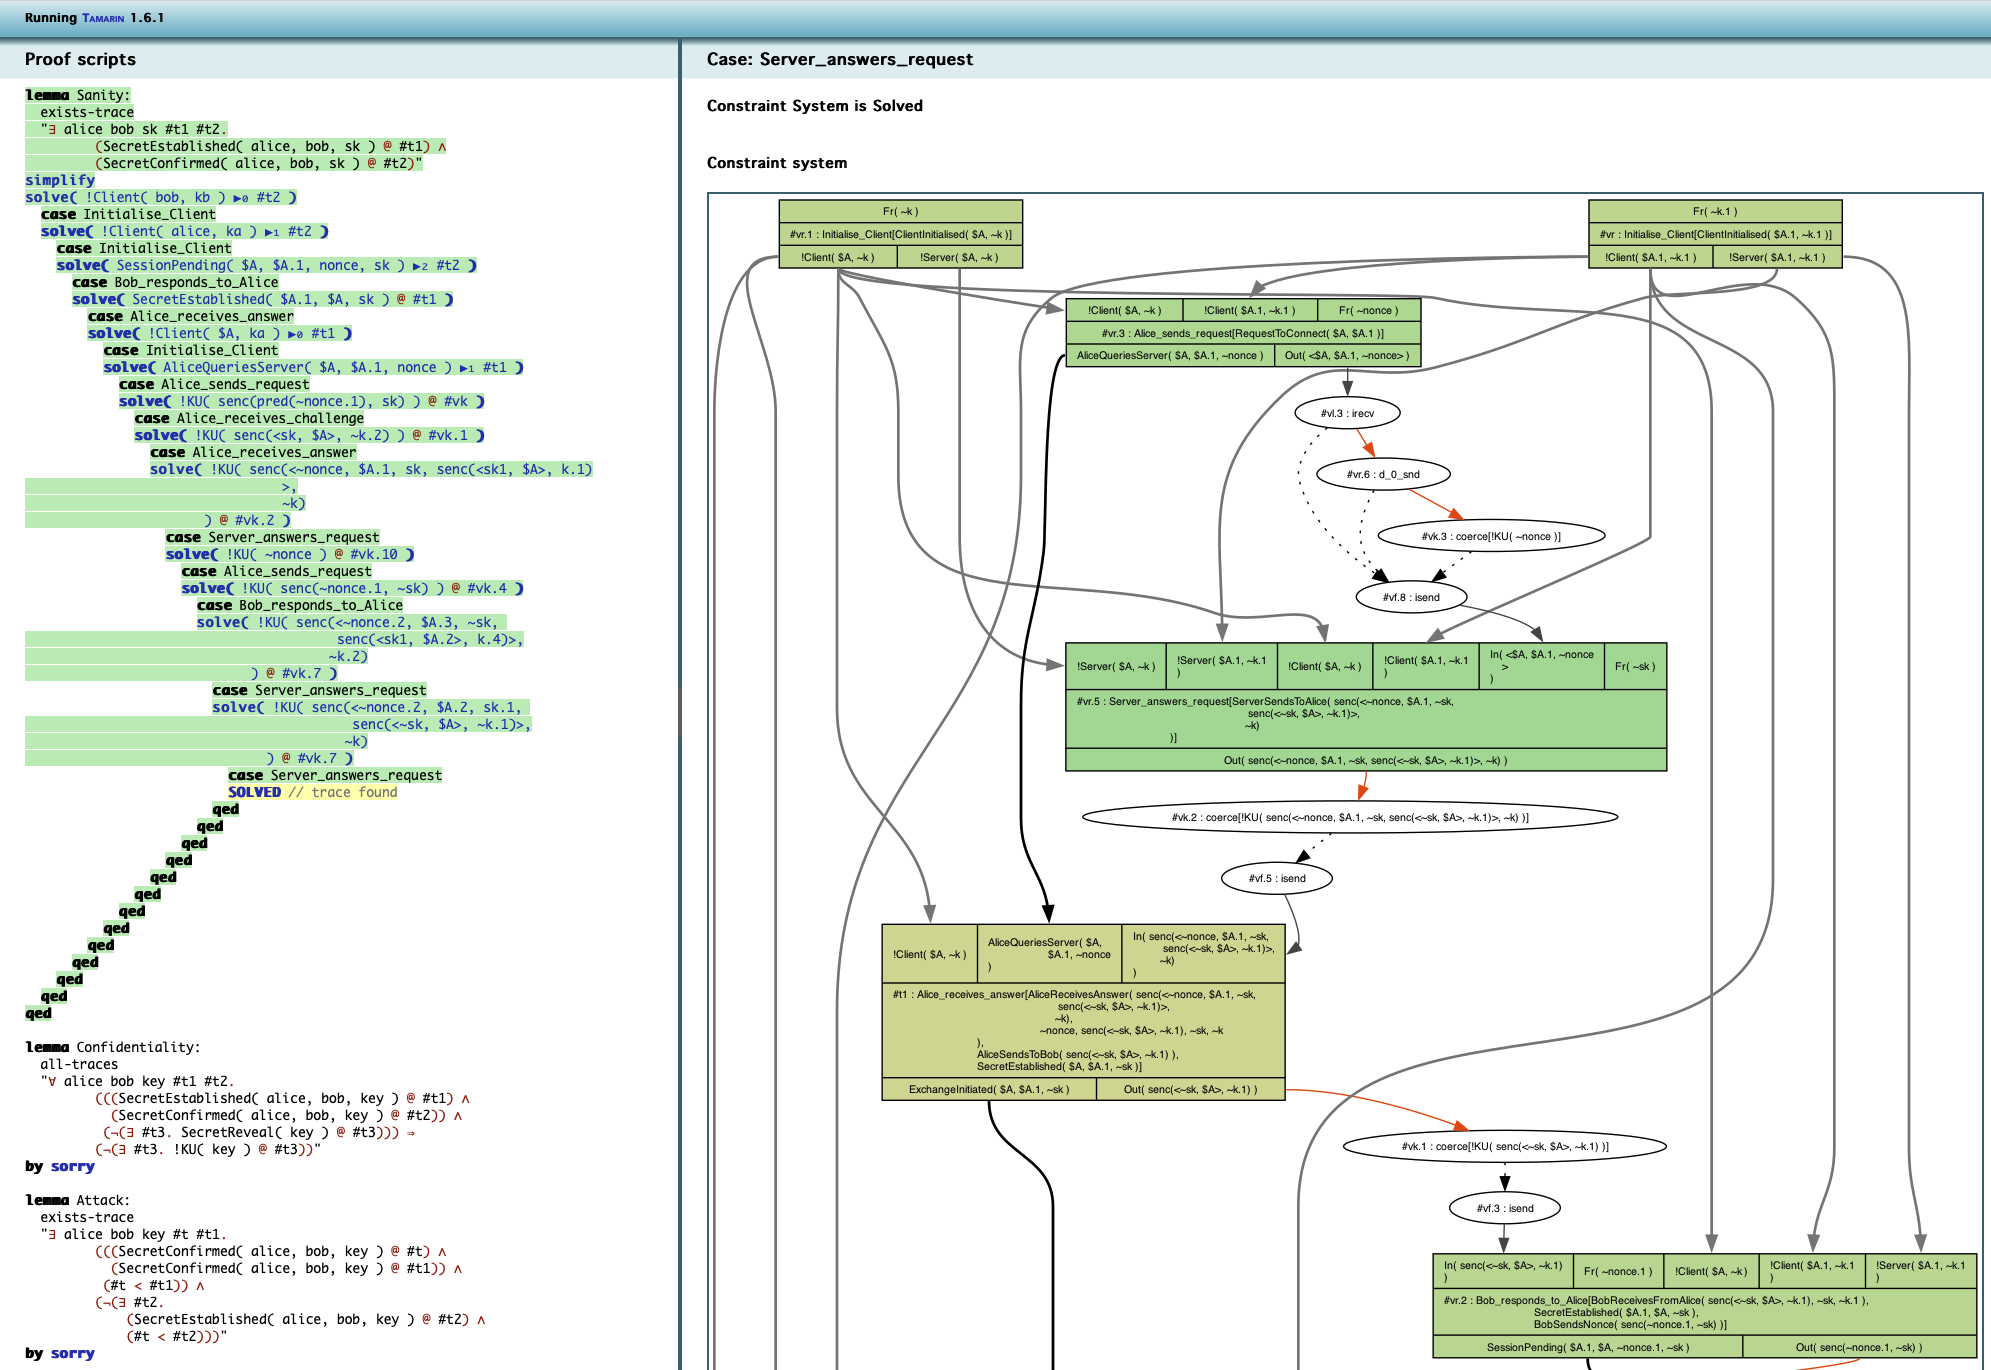
\includegraphics[width=1\textwidth]{Figures/tamaringui.png}
    \caption{Tamarin's interactive mode. The graph on the right displays an intermediate constraint system, while the tree on the left provides the summary of the proof steps performed. Since the investigated property is an existentially-quantified formula and the outcome of the proof is positive, the constraint system must be a valid $P$-solution.}
    \label{fig:interactive}
\end{figure}

\subsubsection{Different Heuristics and Custom Oracles}

During proof-search, Tamarin uses its built-in \textit{smart} heuristic (consult the relevant section of the manual~\cite{tamarinManual} for additional details) to sort the list of intermediate constraint systems to refine. However sometimes the algorithm prioritizes the wrong goals, leading to loops in the search and thus to non-termination. To provide an alternative to the Depth First Search-based standard heuristic, Tamarin also offers multiple variations of the \textit{consecutive} heuristic. This approach is based upon Breadth First Search and prevents starvation by ensuring that no goal is indefinitely delayed. However, this heuristic often produces bigger proofs, while also does not guarantee to terminate.

Additionally, by knowing how to precisely manually guide the search (for example after doing some practice with the built-in interactive mode), users can develop an external \textit{oracle} in any programming language of choice. This oracle is automatically executed by the prover to determine the correct constraint to refine within a list of intermediate goals. The user-defined software receives the name of the lemma and the indexed goal list (as sorted by the smart heuristic) as input, and returns the re-ranked list (or, alternatively, only its first element) as output. Note that oracles are generally stateless: for each step of the proof, the program is executed from scratch, with only the name of the considered lemma and the list of current security goals as input.

\subsubsection{Restrictions}

Similarly to lemmas, \textit{restrictions} are specified through first order logic formulae. They are meant to limit the traces of a protocol considered in the proof search. A Tamarin \textit{theory} is a sextuple $(\Sigma, E, P, \vec{\alpha}, \vec{\phi}, \vec{\psi})$, where $\Sigma$ is a signature, $E$ is an equational theory based on $\Sigma$, $P$ is a set of protocol rules, and $\vec{\alpha}, \vec{\phi}, \vec{\psi}$ are sequences of closed formulae: restrictions, validity claims and satisfiability claims. A theory is true if all of its claims hold for the traces of $P \cup MD$ satisfying the restrictions:
\begin{align*}
    P \cup MD &\vDash \left( \bigwedge_{\alpha \in \text{set}(\vec{\alpha})} \alpha \right) \implies \phi &&\forall \phi \in \text{set}(\vec{\phi})\\
    P \cup MD &\vDash \left( \bigwedge_{\alpha \in \text{set}(\vec{\alpha})} \alpha \right) \land \psi &&\forall \psi \in \text{set}(\vec{\psi})
\end{align*}

An example of restriction usage might consist of avoiding the application of the same rule twice:
\begin{gather*}
    [\texttt{OldFact}(x)] \xrightarrow{\texttt{OnlyOnce}()} [\texttt{NewFact}(x)]\\
    \phi : \forall i,j  \ . \ \texttt{OnlyOnce}() @ i \land \texttt{OnlyOnce} @ j \Rightarrow i = j
\end{gather*}

\subsubsection{Re-use lemmas}

Finally, the last functionality we introduce is \textit{re-use lemmas}: defined with the $\texttt{[reuse]}$ keyword, these formulas, once proved, can be used by Tamarin in the demonstration of the subsequently specified lemmas.